% ============================================================
%  BUFFER gate - board-level wiring diagram.
%  A buffer has no parts of its own: it is just TWO finished
%  NOT-gate boards chained together (output of the first into
%  the input of the second):
%        A -> [NOT] -> A-bar -> [NOT] -> Y = A
%  Build the NOT gate twice (each = one 2N3904 + one 2N3906),
%  share one +5 V rail and one GND, then wire them as below.
%  Compile:  pdflatex wiring.tex
% ============================================================
\documentclass[border=16pt]{standalone}
\usepackage{circuitikz}
\usepackage{tikz}
\usetikzlibrary{calc}

\begin{document}
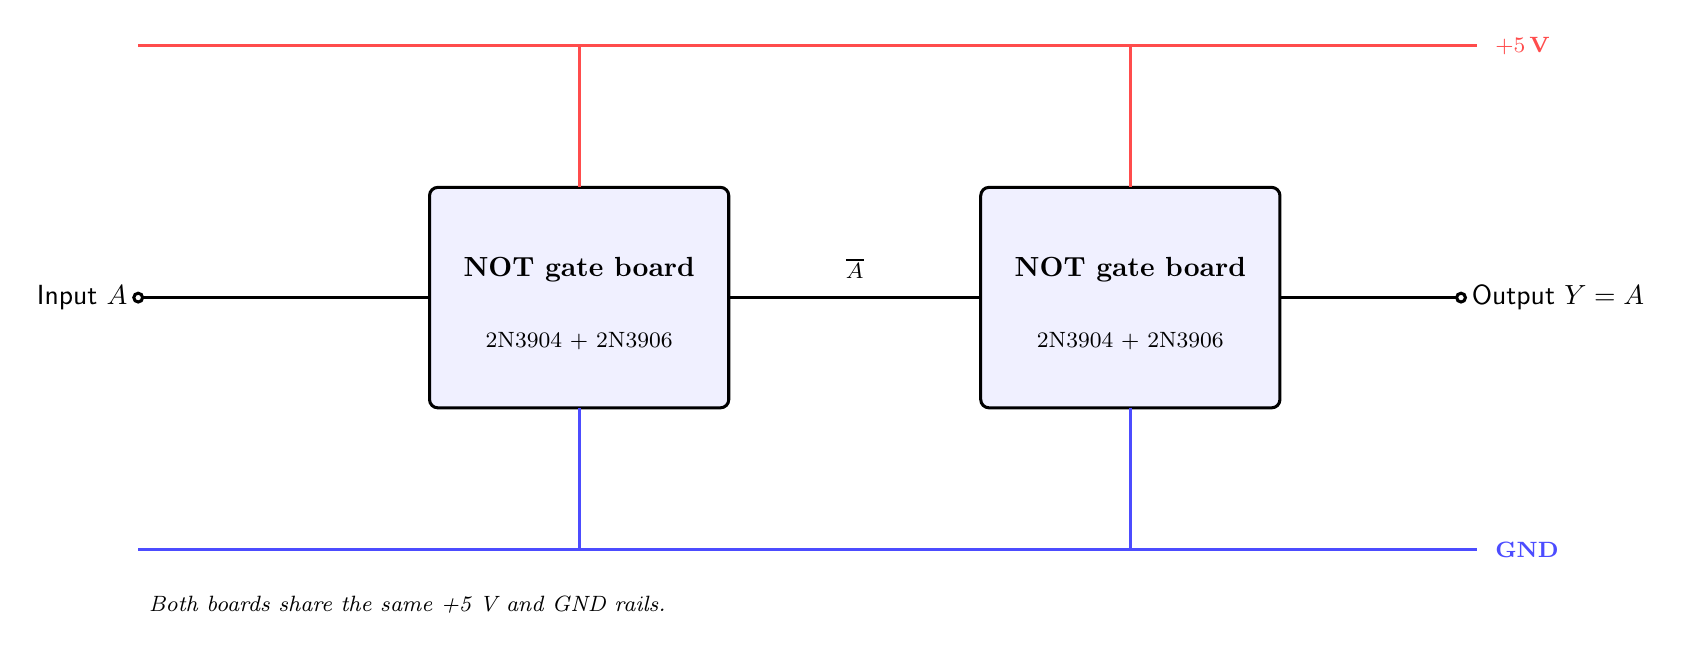
\begin{tikzpicture}[line width=1.1pt, font=\sffamily]

  % ---------- shared power rails ----------
  \draw[red!70]  (-1.5,3.2) -- (15.5,3.2);
  \node[red!70,anchor=west,font=\footnotesize\bfseries] at (15.6,3.2) {$+5\,$V};
  \draw[blue!70] (-1.5,-3.2) -- (15.5,-3.2);
  \node[blue!70,anchor=west,font=\footnotesize\bfseries] at (15.6,-3.2) {GND};

  % ---------- the two NOT-gate boards ----------
  \draw[rounded corners=3pt, fill=blue!6] (2.2,-1.4) rectangle (6.0,1.4);
  \node[align=center, font=\bfseries] at (4.1,0.35) {NOT gate board};
  \node[align=center, font=\footnotesize] at (4.1,-0.55) {2N3904 + 2N3906};

  \draw[rounded corners=3pt, fill=blue!6] (9.2,-1.4) rectangle (13.0,1.4);
  \node[align=center, font=\bfseries] at (11.1,0.35) {NOT gate board};
  \node[align=center, font=\footnotesize] at (11.1,-0.55) {2N3904 + 2N3906};

  % ---------- signal wiring ----------
  \draw (-1.5,0) node[ocirc]{} node[left]{Input $A$} -- (2.2,0);
  \draw (6.0,0) -- (9.2,0);
  \node[above,font=\footnotesize] at (7.6,0.1) {$\overline{A}$};
  \draw (13.0,0) -- (15.3,0) node[ocirc]{} node[right]{Output $Y=A$};

  % ---------- power taps to each board ----------
  \foreach \x in {4.1,11.1}{
    \draw[red!70]  (\x,1.4) -- (\x,3.2);
    \draw[blue!70] (\x,-1.4) -- (\x,-3.2);
  }

  % ---------- note ----------
  \node[anchor=west,font=\footnotesize\itshape] at (-1.5,-3.9)
        {Both boards share the same +5 V and GND rails.};

\end{tikzpicture}
\end{document}
